\documentclass[12pt,twoside]{jreport}  % 文字サイズは12pt, twoside:左右の上にページ番号表示
\usepackage{colortbl}                  % 表に色付けたりする
\usepackage{thesis}                    % 論文用スタイル
\usepackage[dvipdfmx]{graphicx}         % PNG形式の図などを貼りつけられる, 使わないなら外してOK
\usepackage{url}
\usepackage{amsmath}
\renewcommand{\bibname}{参考文献}      % jreportだと"関連図書"になるので強制的に修正

\begin{document}
% タイトルページ
\begin{titlepage}
\begin{center}
\Large

平成yy年度 修士論文\\
\vspace*{3zh}

題 目 \\

\vspace*{3zh}

{\Huge
  論文タイトル\\
}

\vspace*{2zh}

{\Large\bf
  english title\\
}

\normalsize
\vspace*{2zh}

平成yy年2月dd日\\

\vspace*{2zh}


徳島大学大学院 先端技術科学教育部\\
システム創生工学専攻 知能情報システム工学コース\\

\vspace*{3zh}

\begin{table} [h!]
  \centering
  \begin{tabular} {cl}
      学籍番号 & 5000370000\\
      提出者 & 氏 名
  \end{tabular}
\end{table}

\Large
\vspace*{3zh}

\underline{主査             {\normalsize 印}}

\vspace*{1zh}

\underline{副査             {\normalsize 印}}

\vspace*{1zh}

\underline{副査             {\normalsize 印}}

\vspace*{5mm}
\end{center}
\end{titlepage}

\pagenumbering{roman}  % ページ番号表記を小文字のローマ数字に
\setcounter{page}{1}   % ページ番号を1ページに修正
\tableofcontents       % 目次を表示
\listoffigures         % 図目次
\listoftables          % 表目次
\newpage

%%%%%%%%%%%%%%%%%%%%%%%%%%%%%%%%%%%%%%%%%%%%%%%%%%%%%%%%%%%%%%%%%%%%%%%%%

% ここから1ページ
\pagenumbering{arabic}   % ページ番号表記をアラビア数字に
\setcounter{page}{1}     % ページ番号を1ページに修正
%\setlength{\baselineskip}{20pt} % 行間隔を広くする

% ここから本文
\setlength{\baselineskip}{20pt}

% 1章
\chapter{序論}\label{abst}
\section{背景と目的}
本文を書いていく.引用するときはciteを使う->\cite{cite_1}.
citeの文字列はdocument.txtの参考文献の文字列と合わせる.
すると自動的に番号を振ってくれる.

段落分けする場合はこのように空行を挟む.

画像を張る場合は以下のように記述する.

\begin{figure}[htbp]
  \begin{center}
    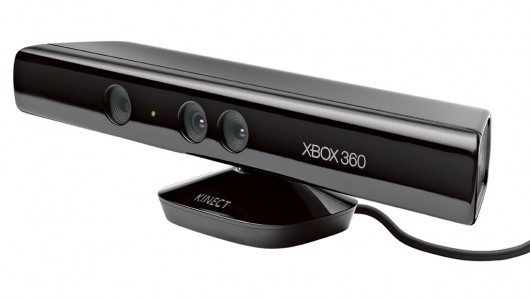
\includegraphics[clip,width=7.0cm]{./images/Kinect.jpg}
    \caption{Kinect}
    \label{fig:Kinect}
  \end{center}
\end{figure}

図ooと文中で用いる場合はrefを使用する->図\ref{fig:Kinect}.
図のlabelとrefの文字列を合わせることで自動的に番号を振ってくれる.
includegraphicsの./images/ファイル名を変更することで表示する画像を変更できる.
使用できる画像は.jpgと.pngのみ.

\section{論文構成}
論文構成を書いていく.


% 章を追加する場合は
% \chapter{関連研究}\label{2nd.tex}
\section{背景と目的}
本文を書いていく.引用するときはciteを使う\cite{cite_1}.
citeの文字列はdocument.txtの参考文献の文字列と合わせる.
すると自動的に番号を振ってくれる.

段落分けする場合はこのように空行を挟む.

画像を張る場合は以下のように記述する.

\begin{figure}[htbp]
  \begin{center}
    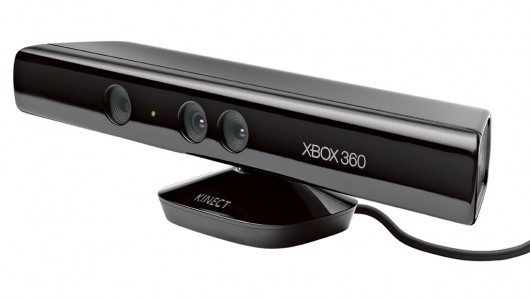
\includegraphics[clip,width=7.0cm]{./images/Kinect.jpg}
    \caption{Kinect}
    \label{fig:Kinect}
  \end{center}
\end{figure}

図ooと文中で用いる場合はrefを使用する図\ref{fig:Kinect}.
図のlabelとrefの文字列を合わせることで自動的に番号を振ってくれる.
includegraphicsの./images/ファイル名を変更することで表示する画像を変更できる.
使用できる画像は[.jpg .png .eps]のみ.

\section{論文構成}
論文構成を書いていく.

% のようにinputを使う

% 結論
\chapter{結論}\label{conclusion}
結論をしっかりかく


% 謝辞
\newpage
\addcontentsline{toc}{chapter}{謝辞}
\chapter*{謝辞}
ありがとう


% 参考文献
\newpage

\addcontentsline{toc}{chapter}{参考文献}
\begin{thebibliography}{99}% ここに参考文献を追加
\bibitem{cite_1} name1, name2, "paper title", confarenceName
\end{thebibliography}

\end{document}

